\documentclass[]{article}
\usepackage{lmodern}
\usepackage{amssymb,amsmath}
\usepackage{ifxetex,ifluatex}
\usepackage{fixltx2e} % provides \textsubscript
\ifnum 0\ifxetex 1\fi\ifluatex 1\fi=0 % if pdftex
  \usepackage[T1]{fontenc}
  \usepackage[utf8]{inputenc}
\else % if luatex or xelatex
  \ifxetex
    \usepackage{mathspec}
  \else
    \usepackage{fontspec}
  \fi
  \defaultfontfeatures{Ligatures=TeX,Scale=MatchLowercase}
\fi
% use upquote if available, for straight quotes in verbatim environments
\IfFileExists{upquote.sty}{\usepackage{upquote}}{}
% use microtype if available
\IfFileExists{microtype.sty}{%
\usepackage{microtype}
\UseMicrotypeSet[protrusion]{basicmath} % disable protrusion for tt fonts
}{}
\usepackage[margin=1in]{geometry}
\usepackage{hyperref}
\hypersetup{unicode=true,
            pdfborder={0 0 0},
            breaklinks=true}
\urlstyle{same}  % don't use monospace font for urls
\usepackage{graphicx,grffile}
\makeatletter
\def\maxwidth{\ifdim\Gin@nat@width>\linewidth\linewidth\else\Gin@nat@width\fi}
\def\maxheight{\ifdim\Gin@nat@height>\textheight\textheight\else\Gin@nat@height\fi}
\makeatother
% Scale images if necessary, so that they will not overflow the page
% margins by default, and it is still possible to overwrite the defaults
% using explicit options in \includegraphics[width, height, ...]{}
\setkeys{Gin}{width=\maxwidth,height=\maxheight,keepaspectratio}
\IfFileExists{parskip.sty}{%
\usepackage{parskip}
}{% else
\setlength{\parindent}{0pt}
\setlength{\parskip}{6pt plus 2pt minus 1pt}
}
\setlength{\emergencystretch}{3em}  % prevent overfull lines
\providecommand{\tightlist}{%
  \setlength{\itemsep}{0pt}\setlength{\parskip}{0pt}}
\setcounter{secnumdepth}{0}
% Redefines (sub)paragraphs to behave more like sections
\ifx\paragraph\undefined\else
\let\oldparagraph\paragraph
\renewcommand{\paragraph}[1]{\oldparagraph{#1}\mbox{}}
\fi
\ifx\subparagraph\undefined\else
\let\oldsubparagraph\subparagraph
\renewcommand{\subparagraph}[1]{\oldsubparagraph{#1}\mbox{}}
\fi

%%% Use protect on footnotes to avoid problems with footnotes in titles
\let\rmarkdownfootnote\footnote%
\def\footnote{\protect\rmarkdownfootnote}

%%% Change title format to be more compact
\usepackage{titling}

% Create subtitle command for use in maketitle
\providecommand{\subtitle}[1]{
  \posttitle{
    \begin{center}\large#1\end{center}
    }
}

\setlength{\droptitle}{-2em}

  \title{}
    \pretitle{\vspace{\droptitle}}
  \posttitle{}
    \author{}
    \preauthor{}\postauthor{}
    \date{}
    \predate{}\postdate{}
  

\begin{document}

\doublespacing

\section{Purpose of the study}
\label{sec:Purpose of the study}

The purpose of this research is to apply a generalised linear model
(GLM) suitable for exposure-based operational risk (EBOR) treatments
within the operational risk management framework (ORMF), effectively
replacing historical loss severity curves obtained from historical loss
counts, by forward-looking measures using event frequencies based on
actual operational risk (OpRisk) exposures. Preliminary work on EBOR
models was undertaken by {[}@einemann2018operational{]}. Secondly, this
study provides a comprehensive computational comparison of various
data-intensive techniques amongst each other, and versus
\emph{classical} statistical estimation methods for classification and
regression performances.\medskip

Our understanding of existing ORMF to date is limited to the assumption
that financial institutions (FI's) are risk-neutral: In lieu of the
afore-mentioned this study finally seeks to invalidate the risk-neutral
assumption by means of evidence-based discoveries revealed through a
clustering algorithm arising naturally in the unknowns of the data by
means of a prescribed model, which applies unsupervised learning
techniques to determine what is going on, proposing that FI's are more
risk-averse. This determination is best understood analysing subtle
patterns between data features and trends in the allocated risk capital
estimates. In theory, a risk manager who experiences
persistent/excessive losses due to particular risk events, would
over-compensate cover for these particular risk types, and this would
show in reduced losses in data for these event types over time.

\section{Fundamentals of ORMF's}
\label{sec:Fundamentals of ORMF's}

Congruent to @cruz2002modeling, in the current study the researcher
alludes to the notion that most banks' estimates for their risk's are
divided into credit risk (50\%), market risk (15\%) and OpRisk (35\%).
@cruz2002modeling postulates that OpRisk, which focuses on the human
side of risk management is difficult to manage with the reduced ability
to measure it. The process of that risk, that is the how, manifests in
the conscious and/or unconscious states of mind of the risk practitioner
{[}@hemrit2012major{]}, and encompasses approaches and theories that
focus on how they will choose when faced with a decision, based on how
comfortable they are with the situation and the variables that are
present.

\begin{definition}
\emph{\textbf{Operational Risk} (OpRisk) is defined as:} The risk of loss resulting from inadequate or failed internal processes, people and systems, and from external events. This definition includes legal risk, but excludes strategic and reputational risk.\medskip
\end{definition}

{[}@risk2001supporting{]}.

\section{A theoretical foundation for operational risk}
\label{sec:A theoretical foundation for operational risk}

The major managerial concern for businesses is in the lack of
universally accepted ways to identify their OpRisk, and hence the
inability to successfully account for their susceptibility to this,
particularly following a number of very costly and highly publicized
operational events that lead to catastrophic losses for the banks in
question. OpRisk became popular following a now famed fraudulent trading
incident which was responsible for catastrophic losses that lead to the
collapse of Barings Bank (the UK's oldest bank) in 1995. The term
\emph{OpRisk} began to be used extensively after the afore-mentioned and
similar types of OpRisk events became common.\medskip

A \emph{rogue} trader, Nick Leeson {[}@panjer2006operational{]} risked
the banks' survival rather than expose his trading losses by consciously
deceiving senior management to hide unethical rogue trading acts, was
found responsible for unethical trading practices when he created
illegal trades in his account. He then used his position in the front
and back offices of the bank to hide his losses. Worse still, he went
further in his fraudulent activities incurring greater risks to the
bank, by lying in order to give a false impression of his profits. This
supports the behavoural notion alluded to by @shefrin2016behavioral,
that in most risk-bearing decision-making situations people would rather
incur greater risks to hold on to their current position and things they
already have, than the risks they would have taken to get into that
position in the first place.\medskip

It was later discovered that Nick was placing illegal bets in the
Asian-markets, while covertly keeping these contracts out of sight from
senior management to cover up his illegal trading activities. When his
fraudulent behaviour was discovered (after an earthquake hit at Kobe in
Japan, that collapsed the Osaka Securities Exchange) he succumbed to
unrecoverable losses due to trading positions he had accumulated which
resulted in a loss of around \pounds 1.3 billion to the bank, thus
resulting in it's collapse {[}@martin2009risk{]}. In most, if not all of
case involving OpRisk hazard, human error is at the center of the chain
of events that lead or may lead to OpRisk losses.\medskip

Since then, there have been a series of destructive events worldwide
that have threatened the stability financial systems due to OpRisk
losses. Hefty fines worthy of bankrupting entire corporate entities
often have to be imposed on the guilty culprits sometimes resulting in
irreparable damage to banks' overall business and reputations, such that
widespread regulatory scrutiny has been heightened as a result of a
number of scandalous operational events. @orxablr2018 recognise from
information offered via the operational riskdata exchange (ORX) global
banking loss database that historically, gross loss sizes have been
predominantly high and volatile, characterised by a period (from 2011 to
2016) driven by the occurence of large loss events. This coincides with
the afore-mentioned post-crisis period, predominantly in 2012, followed
by a comparatively stable period in 2017 where industry Oprisk losses
saw sizes decrease significantly. Figure \ref{bank-oprisk_fig}
illustrates comparative distribution of severity of losses per loss
event type reported from 2011 to 2016 during which major banks suffered
nearly \$210 billion worldwide from Oprisk alone.\medskip

\begin{figure}
\centering
\copyrightbox[b]{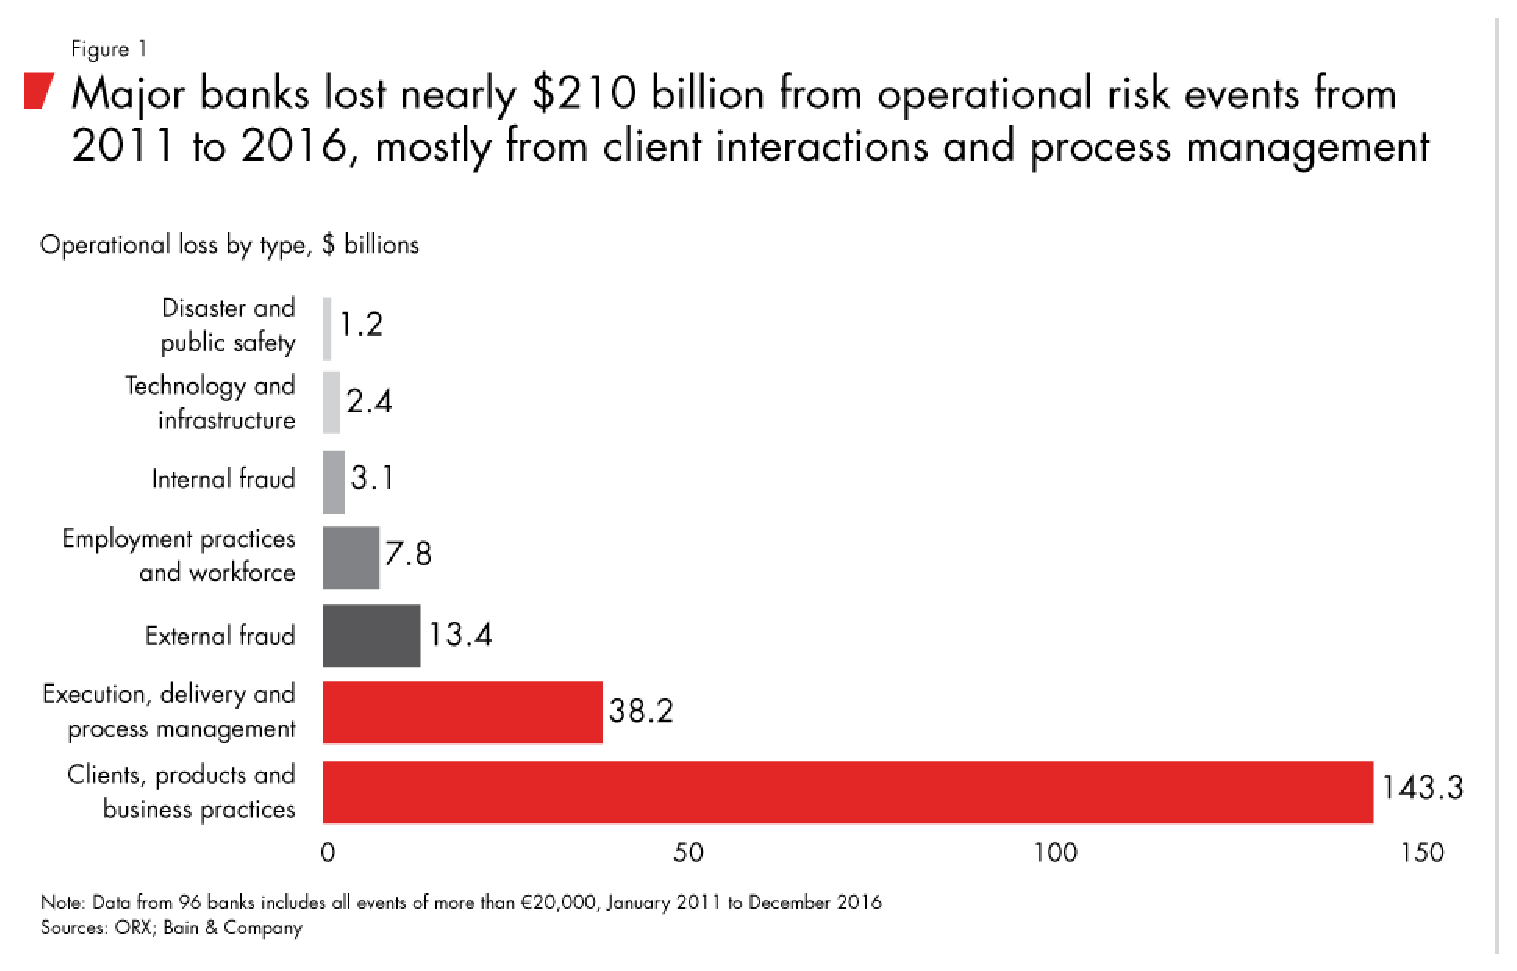
\includegraphics[width=15cm,height=7.5cm]{bank-oprisk_fig1_full.eps}}
             {Source: \url{https://www.bain.com/contentassets/f0199ad9887e402cb37cd1fd316f5ee3/bain_brief_how_banks_can_manage_operational_risk.pdf}}
\caption[Losses suffered from 2011 to 2016 from Oprisk]{Histogram showing a breakdown of gross losses focusing on OpRisk loss events in comparison to each other recorded from 2011 up to and including 2016}
\label{bank-oprisk_fig}
\end{figure}

These OpRisk loss events were due to fraudulent trading activity
consisting of rogue traders dealing in illegally placed high frequency
trades for private clients where prices are hidden. For example, the
January 2016 \lq\lq Dark Pool\rq\rq~trading penalties suffered by
Barclays Bank PLC amounting to about \$70mn and Credit Suisse (\$85mn),
imposed by the United States (US) based securities exchange commision
(SEC). In a case closer to home, @suntimes2019 reports ongoing
investigations launched in April 2015 for price fixing and
``widespread'' collusion between banking insiders in South Africa (SA),
of the market allocation for foreign exchange (FX) currency pairs viz.,
USD/ZAR rates, a case which now has been referred to SA based
competition tribunal for prosecution, as late as February 2017. Three
local banks viz., Absa bank, Standard bank \& Investec are implicated in
the scandal along with 14 others; some of which have already been fined
within juristictions they reside {[}@bustech2017{]}, may be liable to
payment of an admistrative penalty equal to 10\% of their annual
turnover.\medskip

This investigation led by the local based competition commission
uncovered irregularities when rogue traders manipulated the price of the
rand through buying and selling US dollars in exchange for the rand at
fixed prices between 2007 and 2013. According to the competition
commission, currency traders allegedly had been colluding or
manipulating the price of the rand through these buy and sell orders to
change supply of the currency in contravention of the competition act
{[}@suntimes2019{]}.\medskip

These acts compromise risk management's advisory service and pedigree,
and arouse huge interest as, with the SA incident, distorting the rand
value has major implications on the living standards of SA's, felt down
to the man in the street. Furthermore, this kind of behaviour can lead
to catastrophic operational losses resulting is a mismatch between
business' expectations and the value the risk management practice is
delivering, which is prevalent across the world and remains unchanged.
There are many attitudes that can potentially infect organisational
processes, the most persistent of these attitudes stem from human
failings that are exploitable {[}@barberis2003survey{]}; such as the
human conditions' propensity to being deceitful during periods of
distress, thus forming a the basis for a (behavioural) theoretical
foundation of OpRisk management.

\section{The basel committee operational risk management framework}
\label{sec:The basel committee operational risk management framework}

The Bank for International Settlements (BIS) is an organisation
consisting of a group of central bank governors and heads of supervision
of central banks around the world who represent an authority on good
risk management in banking. More specifically, the BIS oversee the
duties of the Basel Committee on Banking Supervision (BCBS)/Basel
Commitee. The role of the BCBS is to set out guidelines on international
financial regulation to cover risks in the banking sector. There are to
date three banking accords from the BCBS under the supervision of the
BIS in dealing with financial regulation viz., Basel I, Basel II \&
Basel III. These accords describe an overview of capital requirements
for financial institutions (FI's) in order to create a level playing
field, by making regulations uniform throughout the world.

\subsection{The Capital Adequacy Accord (Basel I)}

Basel I was established in 1988. Basel I meant that FI's were required
to assign capital for credit risk to protect against credit default. In
1996, an amendment to Basel I imposed additional requirements to cover
exposure due to market risk as well as credit risks. Basel I effectively
minimised rules that favoured local FI's over potential foreign
competitors by opening up global competition so that these banks could
buffer against international solvency. In 2001, the @risk2001supporting
consultative package provided an overview of the proposed framework for
regulatory capital (RC) charge for OpRisk upon the realisation of
financial institutions' (FIs) OpRisk component, which constitutes a
substantial risk component other than credit and market risk. \medskip

A construct for credit risk modelling uses in OpRisk is borne out of the
structural model found in @merton1974pricing, whereby a theory for
pricing corporate debt is presented. @merton1974pricing postulates the
bond's value is dependent on the volatility of the firms value at a
given interest rate i.e., the risk structure of interest rates
{[}@rosa2012litigation{]} under possible gains or losses to investors
when there is a significant (unanticipated) probability of default. This
credit risk model adapted to OpRisk defines what is now called the
\emph{exposure-based} operation risk (EBOR) model. The ultimate task of
defining the ideal \emph{exposure} measure for a operational event data
is specifically dealt with in this study. There are two types of
OpRisk's viz., potential high severity risk where the probability of an
extreme loss is very small but costly, and high frequency/low severity
risk where frequency plays a major role in the OpRisk capital charge
calculation. Many times loss of operational nature are attributed to
credit defaults or market risk related movement.\medskip

Conscequently, @rosa2012litigation founded risk \emph{exposure} for
events of operational nature which triggered off the filing of
litigations, but nevertheless related to credit or market risk losses as
defined by the credit risk or market risk exposures as opposed to
standard OpRisk types whose exposure was undefined. The adaptation to
the OpRisk case, of the @merton1974pricing's concept adapted in
@rosa2012litigation to OpRisk losses involving initial public offerings
(IPO's) requires new types of data which incorporate predictive factors
(using a combination of statistical modeling and scenario analysis),
allowing for buliding this \emph{exposure-based} method.\medskip

After completing the IPO dataset, an EBOR model is expressed as a common
credit risk model:

\textbackslash{}begin(eqnarray) L\_\{EXPECTED\} =
\mbox{probability of litigaion} X L\_\{DEFAULT\}
\textbackslash{}end\{eqnarray\}

Where \(L\) denotes loss. Conceptually, this factor based quantification
model for capital requirements can be extended to also include future
events.

\subsection{New Capital Adequacy Accord (Basel II)}

The framework for Basel II was implemented in June 2006. The rationale
for Basel II is to introduce risk sensitivity through more restrictive
capital charge measures and flexibility with specific emphasis on
OpRisk. The structure of the new accord is built upon a three-pillar
framework: Pillar I stipulates minimum capital requirements for the
calcualtion of regulatory capital for credit risk, market risk and
OpRisk in order to retain capital to ward against these risks. Pillar II
imposes a supervisory review process whereby additional capital
requirements can be imposed; such as the bank's internal capital
assessements or to act on needed adequate capital support or best
practice, for mitigating their risks. Pillar III relates to market
discipline i.e., transparency requirements which require banks to
publicly provide risk disclosures to keep them in line by enabling
investors to form an accurate view of their capital adequacy, in order
to reward or punish them on the basis of their risk profile.\medskip

Basel II describes three methods of calculating capital charge for
OpRisk RC viz., the standardised approach (SA), the basic indicator
approach (BIA) and the internal measurement approach (IMA). The basic
indicator approach (BIA) sets the OpRisk RC equal to a percentage (15\%)
of the annual gross income of the firm as a whole to determine the
annual capital charge. The SA is similar to the BIA except the firm is
split into eight business lines and assigned a different percentage of a
three year average gross income per business line, the summation of
which is the capital charge {[}@hoohlo2015new{]}. In the IMA, the bank
uses it's own internal models to calculate OpRisk loss.

\subsection{Basel III}

Basel III establishes tougher capital standards through more restrictive
capital definitions, higher risk weighted
assets\footnote{Also reffered to as risk-weighted amount, it is a measure of the bank's total credit exposure}
(RWA's), additional capital buffers, and higher requirements for minimum
capital ratios {[}@mysis2013{]}. Through Basel III, the BCBS is
introducing a number of fundamental reforms grouped under three main
headings {[}@basel2010basel{]}: 1{]} A future of more capital through
incremental trading book risk (credit items in trading book treated in
the same way as if they were in banking book), 2{]} More liquidity
through the introduction of a global liquidity risk standard: Basel III
will push banks toward holding greater levels of liquid instruments,
such as government bonds and more liquid corporate instruments, and 3{]}
Lower risk under the new requirements of the capital base i.e.,
establish more standardized risk-adjusted capital requirements.\medskip

The future regulatory environment requires OpRisk professionals who are
not only intelligent, creative and motivated but also have the courage
to uphold the OpRisk advisory service standards. Businesses that want to
successfuly manage OpRisk would be well advised to utilize new
theoretical and empirical techniques such that large and small scale
experiments play an important role in risk analysis and regulatory
research.

\section{Modern OpRisk measurement frameworks (ORMF's)}
\label{sec:Modern OpRisk measurement frameworks (ORMF's)}

Regarding the sequence Basel I and Basel II: Regulation begins as a
qualitative recommendation which requires banks to have an
assets-to-capital multiple of at least 20, then focuses on ratios in
which both on-balance sheet and off-balance sheet items are used to
calculate the bank's total RWA, then on tail risk. In other words,
auditors' discretion is replaced by market perception of capital,
meaning there is a market risk capital charge for all items in the
trading business line, then exciting new static risk management
approaches which involve calculating a 99.9 percentile left tail
confidence interval to measure OpRisk value-at-risk (OpVaR) and convert
it into a RC charge.\medskip

\subsection{Advanced Measurement Approach (AMA)}
\label{sec:Advanced Measurement Approach (AMA)}

The advanced measurement approach (AMA) is an IMA method which applies
estimation techniques of OpRisk capital charge derived from a bank's
internal risk measurement system {[}@cruz2002modeling{]}. Basel II
proposed measurement of OpRisk to define capital requirements against
unexpected bank losses whereas the unexpected loss (UL) is the quantile
for the level \(\alpha\) minus the mean. According to the AMA, which is
thought to outperform the simpler SA approach and the BIA, RC
requirements are defined according to the UL limit in one year and the
loss distribution at a 99.9\% confidence level (\(\alpha = 0.01\%\))
aggegate loss
distribution\footnote{The aggregate loss distribution is obtained by convoluting a loss event frequency distribution and a loss severity distribution by means of the random sums method.}
used as a measure of RC. The BCBS proposes to define RC as \(RC = UL\).
This involves simulations based on historical data to establish
frequency and severity distributions for losses. In this case the RC is
a value-at-risk (VaR) measure.\medskip

\subsubsection{Loss distribution approach (LDA)}
\label{sssec:Loss distribution approach (LDA)}

The loss distribution approach (LDA) model is based on actuarial
techniques and is generally accepted as the industry (AMA) standard for
OpRisk estimation. LDA models require quant level expertise in order for
one to accept the statistical relationships linking the actual
(perceived) risk exposures. What it has done is to provide the most
realistic risk profiles of a company to date
{[}@einemann2018operational{]}, based on partitioning OpRisk loss data
into sufficiently homgeneous sets, typically corresponding to
combinations of business lines (BL) and event types (ET), and to
calibrate a frequency and severity distribution for each BL/ET
combination. LDA models cover risks that are well reflected through
historical events and exposure data is used in several of the steps of
the process in frequency and severity modeling.\medskip

\section{What is exposure?}
\label{sec:What is exposure?}

The formal definition of exposure in risk management is:

\begin{definition}
\textbf{The risk remaining after risk treaments have been applied} i.e., the risk *a priori* to considering the actual experience of the corporation or FI.
\end{definition}

In the OpRisk context, the total OpRisk loss is captured by certain
\emph{exposure} measures, which are quantities that are thought to be
roughly proportional to the overall risk associated with an operational
event or loss {[}@parodi2014pricing{]}. The measure of exposure needed
depends on what loss variable one is attempting at projecting which is
dependent on a varied mix of factors. Specifically in relation to the
LDA model for OpRisk the exposure measure is dependent on whether we are
projecting the aggregate losses (severity) or the number of losses
(frequency). When carrying out this decision making expercise the
following were considered:

\begin{list}{*}{}
\item The availability of historical exposure data over the same period for which the losses are recorded
\item The exposure estimate for future periods
\end{list}
\medskip

In this study, the intensity (rate) of occurance of loss events is the
fundamental unit of of analysis for estimating the number of loss events
(frequency) used for OpRisk loss based on the causal factors for the
business. The causal factors are key to the relationship of the
phenomenona which consists of a problem questioning whether a firm
susceptibility to OpRisk hazard growth results in the degree of OpRisk
losses slowing as a conscequence of enhanced OpRisk controls. As per LDA
model steps, one begins by using Poisson modeling for counts to estimate
the rate loss events (frequency) and the opportunity or exposure for
counting for all available observations over a time lag (\([T,T+\tau]\))
\emph{d}; defined as the \emph{exposure} measure.\medskip

The Basel III capital adequacy rules permit model-based calculation
methods for capital, including the AMA for OpRisk capital. Under Basel
III, standardised methods for OpRisk capital have been overhauled,
however for a while there was no prospect of an overhaul of the AMA.
Given the relative infancy of the field of OpRisk measurement, banks are
mostly free to choose among various AMA principle-based frameworks to a
significant degree of flexibility {[}@risk2016supporting{]}. A bank that
undertakes an AMA should be able to influence their capital requirements
through modeling techniques resulting in lowered pressure on OpRisk
capital levels, which in turn has a positive impact on the bank.\medskip

A FI's ability to determine the framework used for its regulatory OpRisk
RC calculation, evolves from how advanced the FI is along the spectrum
of available approaches used to determine capital charge
{[}@risk2001supporting{]}. BCBS recognizes that a variety of potentially
credible approaches to quantify OpRisk are currently being developed by
the industry, and that these R\&D activities should be incentivised.
Increasing levels of sophistication of OpRisk measurement methodologies
should generally be rewarded with a reduction in the regulatory OpRisk
capital requirement.

\subsection{The standardised measurement approach (SMA)}

The flexibility of internal models was expected to narrow over time as
more accurate OpRisk measurement was obtained and stable measures of RC
were reached, ultimately leading to the emergence of best practice.
Instead, internal models produced wildly differing results of OpRisk RC
capital from bank to bank, contrary to the expectations of the BCBS. In
March 2016, the BCBS published for consultation a standardised
measurement approach (SMA) for OpRisk RC; that proposes to abandon the
freedom of internal modelling (thus ending the AMA) approaches for
OpRisk RC, in exchange for being able to use a simple formula to
facilitate comparability across the industry.\medskip

Under the SMA, RC will be determined using a simple method comprising of
two components: A stylised systemic risk model (business indicator
component), and an idiosyncratic risk model (loss component), which are
combined via an internal loss multiplier (ILM), whose function is to
link capital to a FI's operational loss experience to determine SMA
capital.\medskip

The SMA formula is thought to be consistent with regulators' intent for
simplification and increased comparability across most banks. However,
there is a feeling from some in the banking industry that the SMA is
disadvantaged as it is not the same as measuring OpRisk.
@mignola2016comments and @peters2016should identified that the SMA does
not respond appropriately to changes in the risk profile of a bank i.e.,
it is unstable viz., two banks of the same risk profile and size can
exibit OpRisk RC differences exceeding 100\%, and risk insensitive; that
SMA capital results generally appear to be more variable across banks
than AMA results, where banks had the option of fitting the loss data to
statistical distributions.

\subsection{Argument}
\label{ssec:Argument}

Over the last twenty years, hard-won incremental steps to develop a
measure for the size of OpRisk exposure along with the emergence of
promising technologies presents a unique opportunity for bankers and
treasurers - traditionally risk-averse players - to develop a novel type
of way of looking at decision making under risk/uncertainty. New
technologies have been introduced which make use of up to date technical
solutions (such as homo heuristics developed by @gigerenzer2009homo, who
mainatain their methods solve practical finance problems by simple rules
of thumb, or @kahneman2003perspective's intuitive judgements and
deliberate decision making), argued to more likely represent the true
embedded OpRisk in financial organisations as these methods are designed
to fit normal behavioral patterns in their formulation, which is
consistent with how decisions are made under risk/uncertainty.\medskip 

What are the important steps toward completing the post crisis reforms
during the current year? Should the risk management fraternity follow
the
chartered\footnote{Meaning as of the publication [@risk2016supporting] the methods brought forth in the consultative document have not been approved for the public, the ideas within an experimental (leased) phase for the exclusive use of BCBS and certain FI's}
path followed in the @risk2016supporting consultative document,
scrapping away twenty years of internal measurement approaches (such as
the AMA), or should the focus of financial regulators shift toward
improving on what they see fit within current existing AMA frameworks.
The question is should OpRisk managements' focus be on stimulating
active discussions on practical approaches to quantify, model and manage
OpRisk for better risk management and improved controls, or abandon the
adoption of innovative measurement approaches, such as the AMA, in
exchange for being able to use a simple formula across the whole
industry?

\section{Context of the study}
\label{sec:Context of the study}

Regulatory reforms are designed and fines imposed to protect against
operational errors and other conduct costs connected with wrongdoing and
employee misconduct. Despite the introduction and use of these seemingly
robust strategies, regulations, processes and practices relating to
managing risk in FI's, bank losses continue to occur at a rather
distressing frequency. A cyclical pattern of OpRisk loss events still
persists; as evidenced in the recent price fixing and collusion cases,
defeating the explicit objectives of risk management frameworks. This
demonstrates a scourge of reflexivity prevailing in financial markets
emphasising that, there are theories that seem to work for a time only
to outlive their use and become insufficient for the complexities that
arise in reality.

\subsection{Why \texttt{OpRisk?}}

A forceful narrative in management theory is that an organisation
running effective maintenance procedures combined with optimal team and
individual performers i.e., the right balance of skills in the labour
force and adequate technological advancements, means systems and
services can be used to more efficiently produce material gains, enhance
organisational effectiveness, meet business objectives and increase
investment activity. Conversely, the risk of the loss of business
certainty associated with lowered organisational competitiveness and
inadequate systems technology that underpins operations and services is
a key source leading to a potential breakdown in investment services
activity {[}@hoohlo2015new{]}.\medskip

In fact, OpRisk controls could set banks apart in competition. Consider
the case of a risk practitioner in a financial system who assumes that
he/she is consiously and accurately executing tasks and analysing an
observed subject trusting the validity and relying on visual information
that their sense of sight reveals alone. In the absence of visual
confirmation they are hindered from extracting and/or analysing
information about the system and their efforts to regulate could
potentialy fail. In this scenario, the organisational methods and
functioning of information systems would usually pose shortcomings,
which obscure the full extent of OpRisk challenges from the eyes of the
risk practitioner allowing for operational errors. \medskip

When an attack such as an operational error occurs at a speed that the
OpRisk agent (an individual legal entity or a group) is unable to react
quickly enough, due to limitations of their processing speed, and they
are not able to process all the information in the given time span, they
could lose control/fail of fail in compliance, disincentivising support
for regulation, particularly Basel III recovery and resolution
processes. In latter days more often than not, OpRisk loss cases reflect
lack of sufficient controls being the driver of current OpRisk
management catastrophies. The agent on this end of the spectrum of the
risk management strategy, which mitigates risk and enforces regulation
dependent on visual and information controls is better off than an agent
on the other extreme, who does not react at all to changes in the system
environment.

\section{A new class of EBOR models approach}
\label{sec:A new class of EBOR models approach}

In this study, an important new algorithm for ORMFs and is laid out
coupled with data intensive estimation techniques; viz.~Generalised
Additive Models for locatin Scale \& Shape (GAMLSS), Generalized Linear
Models (GLMs), Artificial Neural Networks (ANNs), Random Forest (RF) \&
Decision Trees (DTs), which have capabilities to tease out the deep
hierarchies in the features of covariates irrespective of the challenges
associated with the non-linear or multi-dimensional nature of the
underlying problem, at the same time supporting the call from industry
for a new class of EBOR models that capture forward-looking aspects.

\section{Problem statement}
\label{sec:Problem statement}

Conventional controls in financial systems where information processing
is slow and have tendencies to rely on manual, uncertain, unpredictable
and unrealistic methods, obscure risk managements' reporting and produce
undesirable pre-market conditions that are vital for operations. The
OpRisk management's function should be able to assist in the ability to
mitigate risks by acquiring and/or refining risk management solutions
which deliver reliable and consistent benefits of improved control and
management of the risks inherent in banking operations {[}@mysis2013{]}.
This proposal attempts to fill the gap in the current system where there
is a risk management information lag or an obstruction from the eyes of
the risk practitioner.

\subsection{Main problem}

The existing models of OpRisk VaR measurement frameworks assume FI's are
risk neutral, and do not learn from past losses/mistakes: We address
weaknesses in current OpRisk VaR measurement frameworks by assuming that
FI's are more risk averse. Furthermore, introducing exposure-based
operational risk modeling, we gain an understanding of how capturing
past losses and exposures of forward looking aspects affect risk
attitudes using machine learning techniques. As a consequence, projected
future losses are estimated through a learning algorithm adapting
capital estimates to changes in the risk profile, i.e.~in the
introduction of new products or changes in the business mix of the
portfolio (e.g.~mergers, trade terminatons, allocations or
disinvestments), providing sufficient incentives for OpRisk management
to mitigate risk.

\section{Objectives of the study}
\label{sec:Objectives of the study}

The research objectives are three-fold:

\subsection{Exposure-based OpRisk (EBOR) models}

To quantify OpRisk losses by introducing generalised additive models for
location, scale and shape (GAMLSS) in the framework for OpRisk
management, that captures exposures to forward-looking aspects of the
OpRisk loss prediction problem. EBOR treatments effectively replace
historical loss severity curves obtained from historical loss counts, by
looking into deep hierarchies in the features of covariates in
investment banking (IB), and by forward-looking measures using event
frequencies based on actual operational risk (OpRisk) exposures in the
business environment and internal control risk factors (BEICF) thereof.

\subsection{Modeling OpRisk depending on covariates}

To investigate the performance of several supervised learning classes of
data-intensive methodologies for the improved assessment of OpRisk
against current \emph{traditional} statistical estimation techniques.
Three different machine learning techniques viz., DTs, RFs, and ANNs,
are employed to approximate weights of input features (the risk factors)
of the model. A comprehensive list of user defined input variables with
associated root causes contribute to the \emph{frequency} of OpRisk
events of the underlying value-adding processes. Moreover, the
\emph{severity} of OpRisk is also borne out through loss impacts in the
dataset . As a consequence of theses new mwthodologies, capital
estimates should be able to adapt to changes in the risk profile of the
bank, i.e.~upon the addition of new products or varying the business mix
of the bank providing sufficient incentives for ORMF to mitigate risk
{[}@einemann2018operational{]}.

\subsection{Interpretation Issues using cluster analysis}

To identify potential flaws in the mathematical framework for the loss
distribution approach (LDA) model of ORM, which is based the derivation
of OpRisk losses based on a risk-neutral measure \(\mathbb{Q}\), by
employing Cluster Analysis (CA). The study addresses weaknesses in the
current \emph{traditional} LDA model framework, by assuming managerial
risk-taking attitudes are more risk averse. More precisely, CA learns
the deep hierarchies of input
features\footnote{A typical approach taken in the literature is to use an unsupervised learning algorithm to train a model of the unlabeled data and then use the results to extract interesting features from the data [@coates2012learning]}
that constitute OpRisk event \emph{frequencies} \& \emph{severities} of
losses during banking operations.\medskip

In theory, a risk manager who experiences persistent/excessive losses
due to particular risk events, would over-compensate cover for these
particular risk types. This would show in reduced losses in those loss
event types over time, subsequently determining whether risk adverse
techniques over-compensate for persistent losses. The wish is to bring
the prescribed model to equilibrium by applying a method that tries to
establish what accurately ascribes to decision rules that people wish to
obey in making predictions about what operational loss events might
result in the future, then use empirical data to test this idea in a way
that is falsifyable.

\section{Significance of the study}
\label{sec:Significance of the study}

This study fills a gap in that advancing OpRisk VaR measurement methods
beyond simplistic and traditional techniques, new data-intensive
techniques offer an important tool for ORMFs and at the same time
supporting the call from industry for a new class of EBOR models that
capture forward-looking aspects of ORM {[}@embrechts2018modeling{]}. The
current \emph{traditional} approach consists of a loss data collection
exercise (LDCE) which suffers from inadequate technologies at times
relying on spreadsheets and manual controls to pull numbers together,
and therefore do not support the use of data intensive techniques for
the management of financial risks. In this study, a new dataset with
unique feature characteristics is developed using an automated LDCE, as
defined by @basel2011operational for internal data. The dataset in
question is at the level of individual loss events, it is fundamental as
part of the study to know when they happened, and be able to identify
the root causes of losses arising from which OpRisk loss
events.\medskip 

This study will provide guidance on combining various supervised
learning techniques with extreme value theory (EVT) fitting, which is
very much based on the Dynamic EVT-POT model developed by
@chavez2016extreme. This can only happen due to an abundance of larger
and better quality datasets and which also benefits the loss
distribution approach (LDA) and other areas of OpRisk modeling. In
@chavez2016extreme, they consider dynamic models based on covariates and
in particular concentrate on the influence of internal root causes that
prove to be useful from the proposed methodology. Moreover, EBOR models
are important due to wide applicability beyond capital calculation and
the potential to evolve into an important tool for auditing process and
early detection of potential losses, culminating in structural and
operational changes in the FI, hence releasing human capital to focus on
dilemmas that require human judgement.

\section{Organisation of the study}
\label{sec:Organisation of the study}

This study consists of seven chapters. Chapter \ref{INTRODUCTION}
outlines the purpose, followed by an overview of the relevance and
importance in the existing work. Then the general concept behind EBOR
models is introduced and an argument is presented of the relevance of a
new class of EBOR models to remediate some of the shortcomings in OpRisk
LDA modeling; coscequently the research problem \& objectives are
stated, followed by an account of significance. The introductory chapter
is succeded by a general literature review Chapter
\ref{LITERATURE REVIEW}, succeeded by three stand alone chapters, the
purpose of each is to provide clarity, based on theory and empirical
evidence, focusing on three specific research objectives each
contributing to resolve specific problems in the OpRisk literature,
given how its importance has become more pronounced in time. In these
chapters the application of machine learning techniques on the observed
data take centre-stage demonstrating how issues in OpRisk capital
requirement estimation are more effectively resolved.\medskip

Chapter \ref{LITERATURE REVIEW} gives an overview of theoretical
foundations of OpRisk, a review of the LDA model, an AMA technique used
in the generation of \texttt{OpVaR}. Then provides a breakdown of why
EBOR models are a promising approach to remediate some of the LDA
shortcomings, furthermore on how EBOR components presented in this study
differ to contrasting papers which demonstrates to value of this paper
by elaborating on the gap it fills in more detail. Chapter
\ref{LITERATURE REVIEW} concludes with a lead up to chapter
\ref{EXPOSURE-BASED OPERATIONAL RISK ANALYSIS} by proposing a research
methodology in which a combination of ML techniques and statistical
theory underlying ORMF's would benefit measurement of capital
requirements for OpVaR.\medskip

Chapter \ref{EXPOSURE-BASED OPERATIONAL RISK ANALYSIS} deals with the
application of EBOR techniques using the GLM and GAMLSS models in more
detail, and the empirical determinants due to the different components
of OpRisk measurement under the new class of EBOR models. The chapter
deals with the analysis of EBOR techniques to the portfolio of a wide
range OpRisk losses found in the dataset and their integration into an
LDA framework.


\end{document}
